The following chapter will show the performances obtained after the MPI integration in our code.
We have benchmarked four different problem sizes:
\begin{itemize}
\item small dimension problem $128\times 128 \times 128$;
\item medium dimension problem $256\times 256\times 512$;
\item large dimension problem $512\times 512\times 1024$;
\item very large dimension problem $4096\times 512\times 512$.  
\end{itemize}
All problems have been tested using 1D and 2D decomposition, so that it is possible to have a comparison among this two methods.
\\
In addition to these tests we have performed a single core benchmark against the original code, at mesh size varying, and a couple of comparisons, selecting a mid-sized grid of points, switching the compiler and the processor architecture.
We want to highlight that all these problems exploit the Hermitian symmetry along the streetwise axis.
\section{Testing environment}
Our test were conducted at CINECA\cite{Cineca}, an Italian academic research center, which host the $19^{th}$ most powerful supercomputers of the TOP500~\cite{top500} of November 2018 list, Marconi, and GALILeO.

We worked on Marconi\cite{marconi:specs} supercomputer, in particular on Marconi-A2 partition.
Marconi structure fuse different partition to reach the peak performance of 20 PFlop/s; in particular our partition is characterized by 3600 nodes, connected through Intel OmniPath\cite{intel:intelmpivsopenmpi} high performance network. Each node host a 68-cores Intel Xeon Phi 7250, code name Knight Landings, and about 100GB of ram. \\
The machine runs on CentOS 7.2, a Linux distribution, and our benchmark code has been compiled using GNU GCC 7.3~\cite{gcc} with OpenMPI 3.0.0~\cite{openmpi}\cite{MPI:standard3}. We have chosen to compile our benchmark code using the GNU Compiler Collection, instead of using proprietary and optimized Intel compilers, to ensure the possibility to carry out code run time comparisons across CPU from different vendors, with different architectures. 
\par
We have tested different flags during the compilation phase, trying to enable different levels of optimization and code vectorization, the most important feature of the Xeon Phi, however the best results, using the GCC compiler, have been achieved using:
\begin{lstlisting}
-O2 -fpic -march=native -std=c99
\end{lstlisting}
This behavior was expected since our code does not include the OpenMP\cite{openmp} features at present time, so the MIC\cite{mic} (Many Integrated Cores) architecture can not exploit such fundamental feature. Furthermore the compiler flags used are general purpose, and does not providing the desired tuning for the Intel Knights Landing processors, thus resulting in lack of performances and efficiency.\\~\par

Further tests have been carried out, selecting the mid-sized mesh, changing the compiler and the processor's architecture.\\
The first comparison have taken place on Xeon Phi processors, switching from GCC compiler to Intel C Compiler 18.0. Such tests have revealed that the latter provide more than 2x faster code. \\
The second tests have taken place at Cineca, using GALILeO~\cite{galileo:specs} instead of Marconi. Such benchmarks let us move from the MIC architecture of the aforementioned processor, towards a more traditional ones.
GALILeO is a supercomputer based on IBM NeXtScale cluster, offers 400 general purpose compute nodes, each ones equipped with two 18-core Intel Xeon E5-2697 v4, running at 2.30GHz. Every node count 128 GB of RAM, which means 8 GB per core, and the network communications rely on Infiniband technology.

\section{Performances measurement description}
In this little section we illustrate the procedures used to compute the performance indexes.\par
The measures were carried out using the same code, compiled once for all the simulations, tested at $tasks$ variations.\par
Attention should be posed on the concepts of $tasks$, $cores$ and $processors$ or $nodes$. The first identify the number of parallel processes of the simulation and is obtained as the product between the other two values:
\begin{equation*}
tasks = n~cores \times processors
\end{equation*}
 As we will see shortly the code exhibit sensible performances variation depending on the number of nodes involved in the simulation and the cores per nodes configuration. \\~\par
We start providing the definition of speedup:
\begin{equation*}
S = \frac{T_{0}}{T_{p}}
\end{equation*}
In this simple equation $T_{0}$ identify the single core runtime, while $T_{p}$ is the runtime associated with the execution of the code on $p$ tasks. \par
The efficiency is calculated starting from the speedup as 
\begin{equation*}
E = \frac{S}{p}.
\end{equation*}
Every simulation of our benchmarks started with the single core run, in order to establish the baseline. \par
The tool designed to catch the runtime is simple and lightweight. It wraps the simulation, save the runtime for every processor and retrive the highest value only.
The following pseudo-code should give an idea of the working principle.

\begin{lstlisting}
	begin = clock();
LOOP forward WHILE time < t_max-deltat/2
	...
	\*Perform simulation*\
	...
REPEAT forward

	end = clock();
	sim_time = (end - begin) / CLOCKS_PER_SEC; 
	max_sim_time=0.0;
	MPI_Allreduce(&sim_time, &max_sim_time,1,MPI_DOUBLE,MPI_MAX,MPI_COMM_WORLD); 
	FILE *ft = fopen("time_out","w");	fprintf(ft, "Simulation performed in %f s", max_sim_time); 	fclose(ft);
\end{lstlisting}



\section{Single core comparison}
Before seeing the multi-cores performance of our code we have performed a benchmark against the original implementation of Quadrio and Luchini~\cite{cpl:presentazione}, which can be considered as a state of the art solver, and our \emph{pencil decomposed} solver. We are particularly  interested in comparing the timings for a \emph{pencil approach} against a slab ones, as the PLS is. For this reason we do not carry out comparison against PLS and our \emph{slab decomposed} algorithm, since they use exactly the same approach to solve the problem, and it is likely to perform in the same time.
The simulations have taken place in Debian, a Linux environment, employing an Intel i5 running at 3.1 GHz.\par
Keeping in mind the two algorithm structures, we expect that CPL perform faster. Despite we already know which code is faster, this test is important to understand how far our code is moving away from the single core optimum. \par
Our benchmark suggested that on a $64^{3}$ simulation, the CPL perform a single time step in 0.29 s, while our code employ 0.36s.
On wider mesh of $128^{3}$ points, the CPL  is still faster, with a time step completed in 2.94s, while the other code employ 3.11s.\par
Our results confirm the predictions and highlighted that, although on little mesh we perform about 24\% slower than the optimum, on a larger grid our gap reduce to be just the 5\%. \par
Increasing again the mesh size to $200^{3}$ points lead to further reduction in time difference, with the CPL that still perform faster, with 8.02s per time step, against the 8.11s per step of our code. This means just 1\% of difference between the two codes per time step.
\begin{figure}
\begin{center}
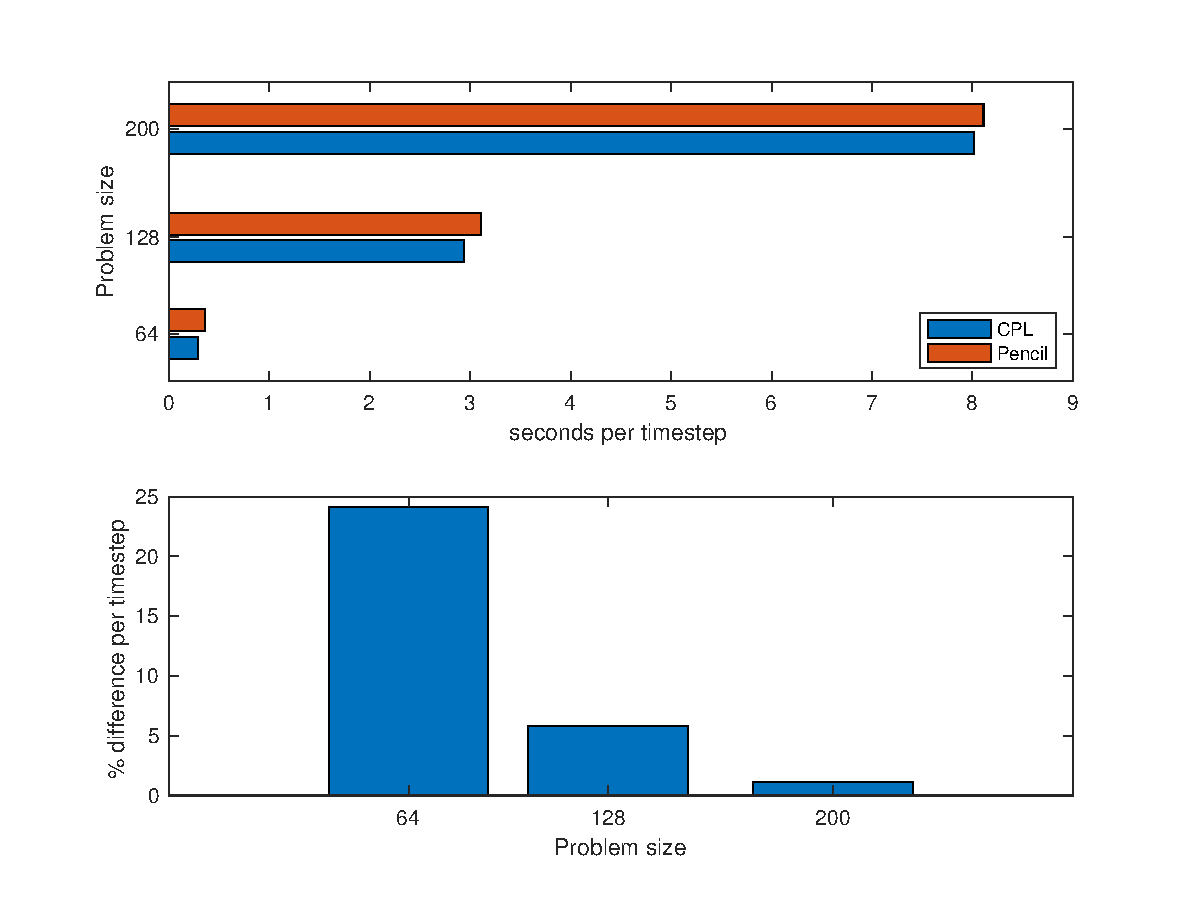
\includegraphics[scale=0.55]{grafici/single_core}
\caption{Single core timing comparison}
\label{single:core}
\end{center}
\end{figure}
On figure~\ref{single:core} are reported the percentage differences and costs per time step of the three tests.



\section{Scaling performance of $128^3$ problem}
We proceed now showing the performances achieved by our code for the small problem.
This is likely the most critical benchmark for our code, since implement a distributed parallel approach to a problem with tiny dimensions could lead to lack of efficiency quickly. 
\par
In this kind of problem the arrays size fits the cache dimension of the Intel Xeon Phi processor; in fact, we achieve greater speedup by using less nodes as possible at cores equality. For this reason in this test we used 64 cores per node. 
\par
The results of figure \ref{641} shows that, although on single core the structure of the slab decomposed algorithm is faster, suddenly the benefits of pencil decomposition overcome the cost due to the poorer array storage.
To understand the latter sentence we should recall the figure of page \pageref{decomposition:example}.
Keeping in mind figure \ref{decomposition:example}, is possibile to understand why the slab decomposition is faster on single core, and typically also for a tiny cores number. Since the slab algorithm work \emph{per plan} we can, wisely, allocate and work just on a small dataset. This affect the communication phase, which will be faster if compared with the ones of the pencil decomposition that, instead, require to allocate all the data at once. 
\par

\begin{figure}
\begin{center}
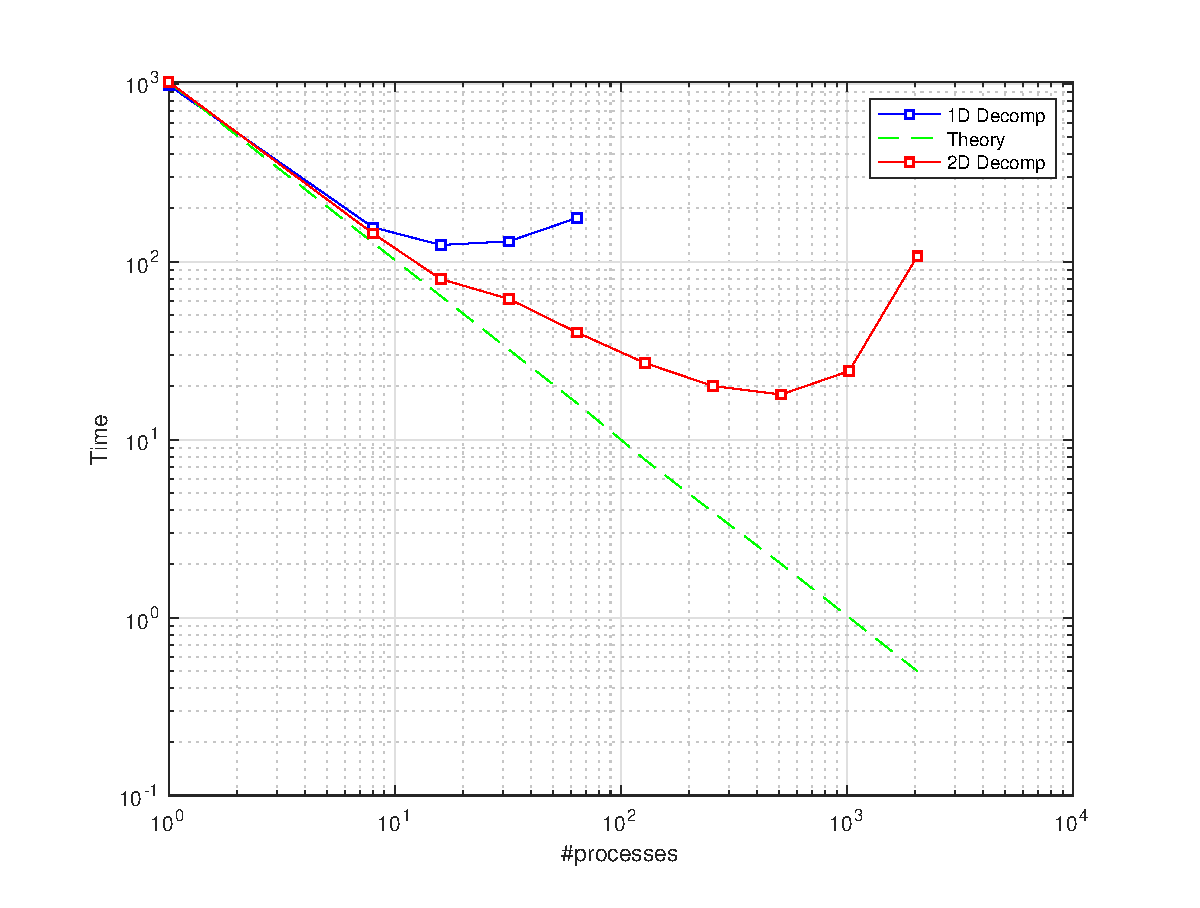
\includegraphics[scale=0.55]{grafici/641}
\caption{Scaling performance of $128^3$ simulation}
\label{641}
\end{center}
\end{figure}

In figure \ref{641} is possible to look at the time needed to perform the DNS, at varying of the cores number and algorithm.
The green dashed line represent the theoretical limit and has been obtained as the ratio between the single core time and the number of cores of the simulation.  \\
Despite of the results could seems poor, the qualitative comparison of figure~\ref{643} against a 3-dimensional FFT, using P3DFFT, reported in \cite[43]{tesi:brach}, suggest that our results are on the average, or better, until the communications cost overcome the benefits of such parallel distributed approach.

\begin{figure}
\begin{center}
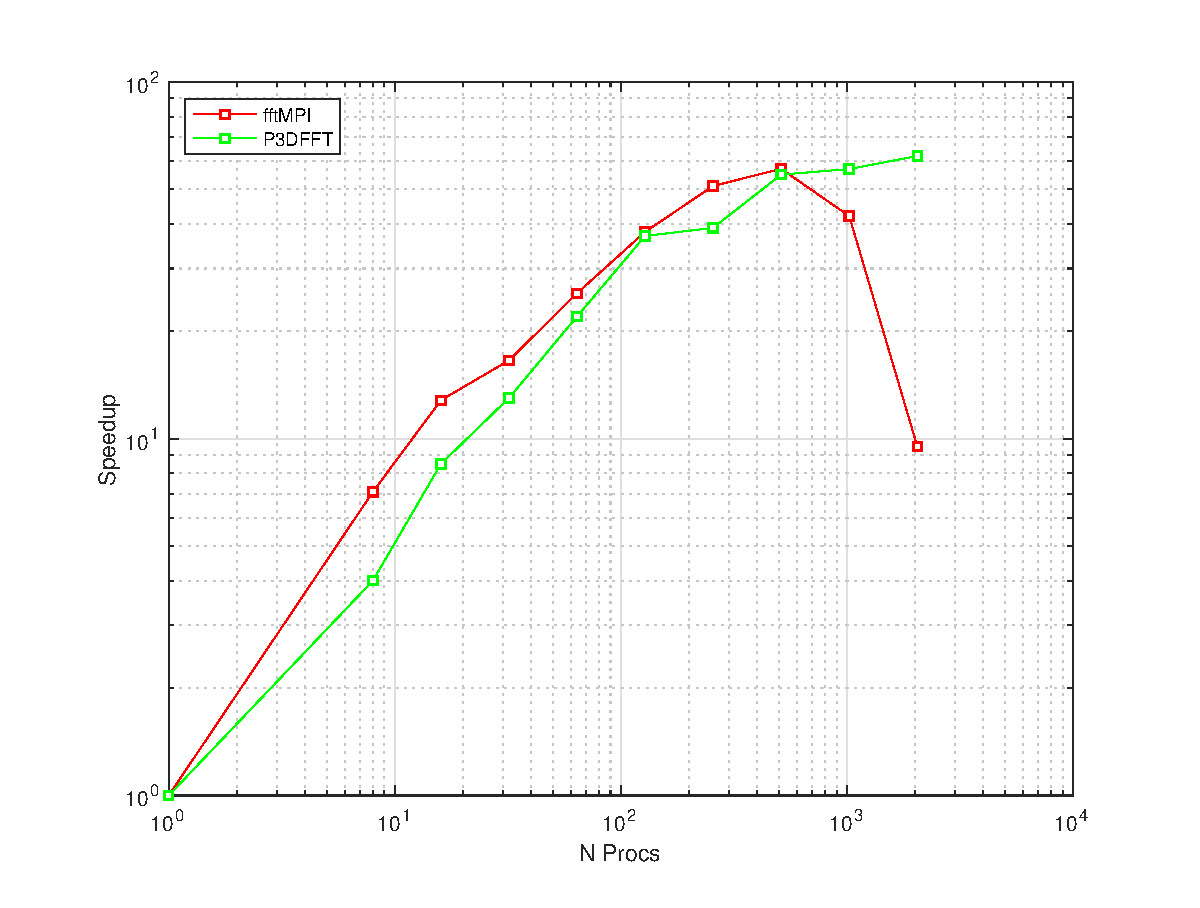
\includegraphics[scale=0.55]{grafici/643}
\caption{Comparison of a 3D FFT against DNS with fftMPI}
\label{643}
\end{center}
\end{figure}

\begin{table}[h]
\caption{Data from $128^{3}$ simulation}
\begin{center}
\begin{tabular}{c c c c c}
\toprule
\textbf{\#Processes} & \textbf{Time [s]} & \textbf{Speedup} & \textbf{Efficiency [\%]} & \textbf{Decomp}\\
\midrule
\multirow{2}{*}{1} & 980 & 1.05 & 100 & 1D\\
& 1022.1 & 1 & 100 & 2D \\
\hline
\multirow{2}{*}{8} & 155.9 & 6.56 & 79 & 1D\\
& 144 & 7.1 & 89 & 2D\\
\hline
\multirow{2}{*}{16} & 124.2 & 8.24 & 49 & 1D\\
& 79.7 & 12.82 & 80 & 2D\\
\hline
\multirow{2}{*}{32} & 130.4 & 7.86 & 24 & 1D\\
& 61.7 & 16.6 & 52 & 2D\\
\hline
\multirow{2}{*}{64} & 176.1 & 5.81 & 9 & 1D\\
& 40 & 25.6 & 40 & 2D\\
\hline
128 & 26.9 & 38 & 30 & 2D\\

256 & 20 & 51.11 & 20 & 2D\\

512 & 17.9 & 57.07 & 11 & 2D\\

1024 & 24.3 & 42.1 & 4 & 2D\\

2048 & 107.3 & 9.52 & 0 & 2D\\
\bottomrule
\end{tabular}
\end{center}
\label{64data}
\end{table}%


The table~\ref{64data} summarizes all data related to the $128^{3}$ simulation. 


\par
According to this table the figure \ref{642} shows the speedup at the varying of the cores number. \\
At the speedup peak the code runs $57$ times faster than serial ones. Such peak is obtained using $512$ cores. However, as expectable, the efficiency of this implementation is quite poor. In fact, if we use more than $16$ cores we drop immediately to performances around $50\%$ or lower. 
For completeness the efficiency behavior is reported in figure \ref{644}.

\begin{figure}
\begin{center}
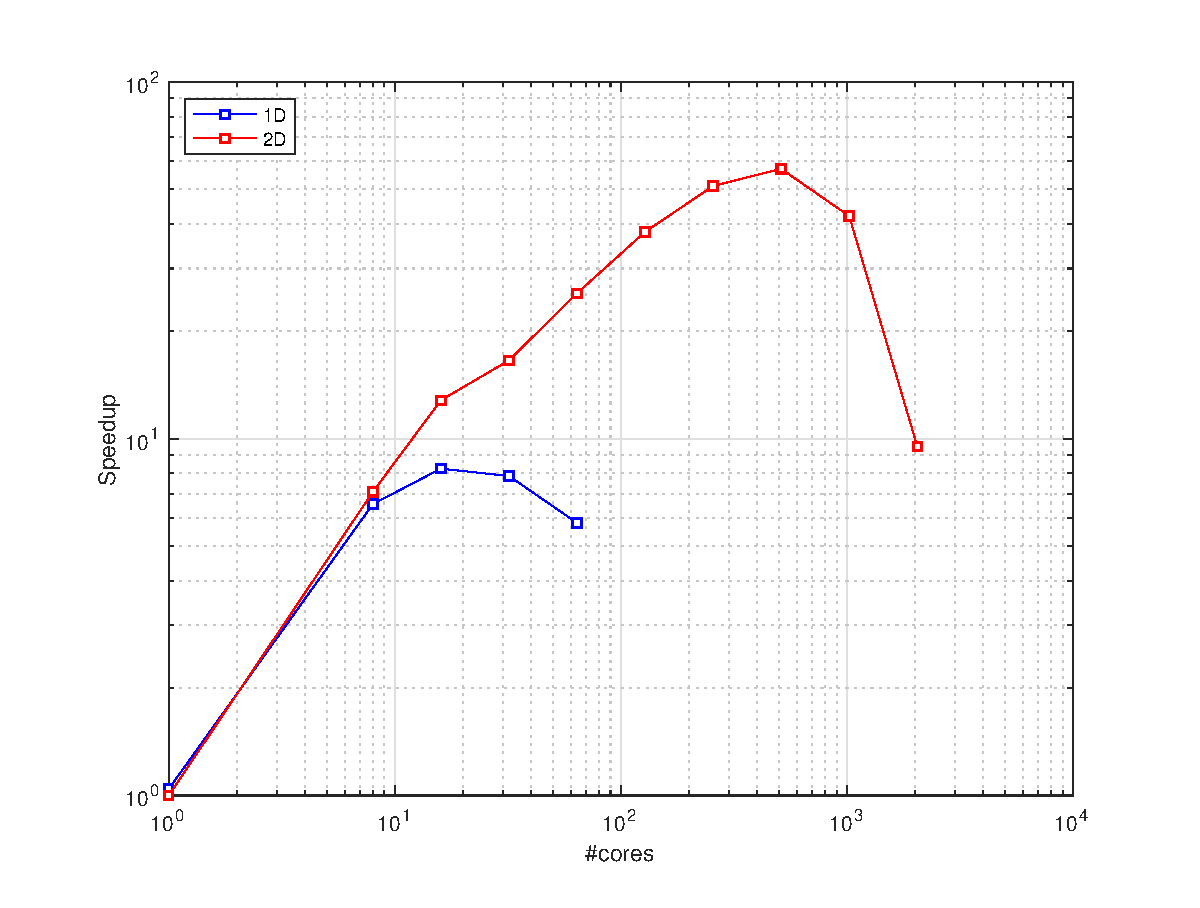
\includegraphics[scale=0.55]{grafici/642}
\caption{Speedup performance factor of $128^3$ simulation}
\label{642}
\end{center}
\end{figure}

\begin{figure}
\begin{center}
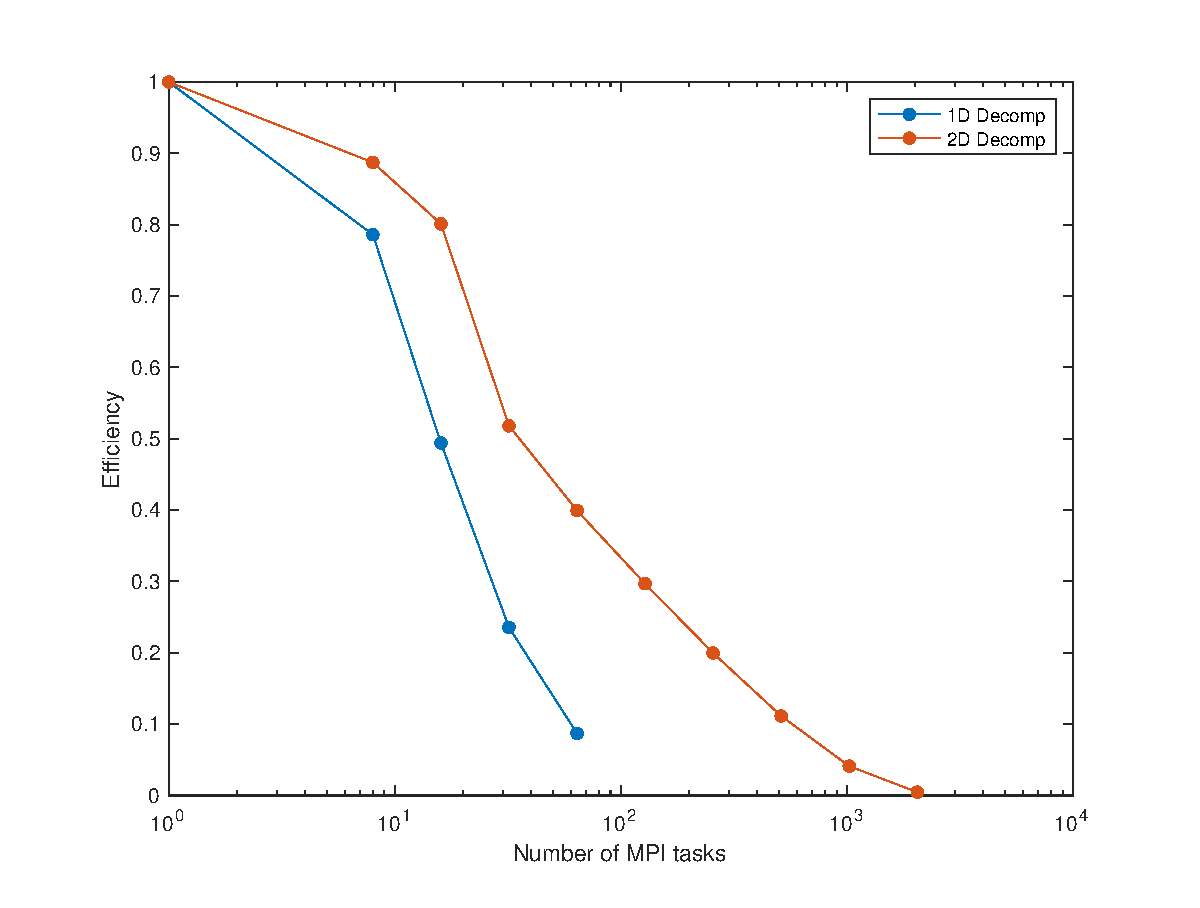
\includegraphics[scale=0.55]{grafici/644}
\caption{Efficiency factor of $128^3$ simulation}
\label{644}
\end{center}
\end{figure}
